\subsection{Requirements Gathering Methodology}

In system development, understanding the customer's way of thinking,
expectations and basic needs are the first major tasks any system developer has to
tackle. Understanding a customer saves time, results in a happier customer,
better reputation, and boosts development productivity. Employing the right
requirements and following up on these should in general keep customers and 
developers on the same page.
Requirements gathering techniques, if applied accurately, will serve as a
suitable preemptive action against incomplete and unclear constantly evolving
requirements. It also forces both parties hold on to the legal and
contractual agreements between a customer and a developer. Here is a list of
industry proven requirements capturing techniques.

\subsubsection{Background reading}

A developer can understand the internal operations, services and cooperation of
a company by reading about the background of the organization. Specialized
tasks, projects, cultures and improvement potential should be 
researched by reading company reports, organizational charts, policy manuals,
job descriptions and documentation of existing systems.

\subsubsection{Interviewing and Questionnaires}

The system analyst interviews the personnel of an organization to understand how
they accomplish their day to day activity. It is very advantageous to gather
firsthand information about priorities, objectives and potential improvements
for the system in perspective of all stake holders including employees and
management. Even though the information gathered from an
interview can be invaluable, it has a tendency to go off topic and be
extremely expensive. Questionnaires can be an alternative way of providing
a goal oriented investigation about the operation of an existing system, 
its current satisfaction among users and suggestions on how to improve it.

\subsubsection{Observation and Document Sampling}

Observation and document sampling is a technique that's effective for captureing
requirements that are impossible to understand through interviews and
questionnaires. It will also enable analysts to gather quantitative data on how
long a task takes to complete in real time. However, observation can be
problematic, requirements that involve sensitive information such as private, 
medical, educational and other protected information can not be handed out to just anyone.

\subsection{MOWAHS Requirement Analysis Framework}
The MOWAHS, MObile Work Across Heterogeneous Systems, a specialized technique
to analyze gathered requirements for mobile work scenario. The framework has
three levels of operation; eliciting scenarios, scenario analysis and
requirement analysis.\cite{wiki:MOWAHS}

\begin{figure}[htb]
	\centering
	 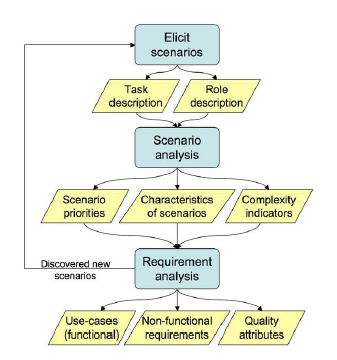
\includegraphics[width=0.8\textwidth]{prestudy/mowahs_style.PNG}
	\caption{MOWAHS Requirements Analysis Style}
	\label{fig:mowahs}
\end{figure}


